\documentclass{article}
\usepackage[utf8]{inputenc}
\usepackage{amsmath}
\everymath{\displaystyle}
\usepackage{biblatex}
\addbibresource{referencias.bib}

\usepackage{hyperref}
\usepackage[spanish, es-tabla]{babel}

\usepackage{authblk}
\renewcommand\Authand{ y }
\renewcommand\Authands{, y }
\renewcommand*{\Authfont}{\bfseries}
%% Page settings
\usepackage[a4paper, margin=1in]{geometry}
\usepackage{graphicx}
\usepackage{multirow}
\usepackage{float}
\usepackage{caption}
\usepackage{subcaption}
\usepackage{lipsum}
\usepackage{wrapfig}
\usepackage{booktabs}
\usepackage{siunitx}
\DeclareSIUnit{\calorie}{cal}
\usepackage{amsmath}
\usepackage{multicol}

\usepackage[table]{xcolor}
\renewcommand{\d}{\text d}
\newcommand{\dd}[2]{\frac{\d #1}{\d #2}}
\newcommand{\ddp}[2]{\frac{\partial #1}{\partial #2}}

\newcommand{\myfigure}[4][0.65]{%
    \vspace{1em}
    \noindent\begin{minipage}{\linewidth}%
        \makebox[\linewidth]{%   For centring figures
            \includegraphics[width=#1\linewidth]{#2}}
        \captionof{figure}{#3}
        \label{#4}
    \end{minipage} 
    \vspace{0.5em}}

\usepackage{amsfonts}
\newcommand{\overbar}[1]{\mkern 1.5mu\overline{\mkern-1.5mu#1\mkern-1.5mu}\mkern 1.5mu}

\title{\vspace{-15mm}\fontsize{24pt}{10pt}\selectfont\textbf{Conductividad Térmica}} % Article title 

\author{Andrés David Rojas Lozano}
\author{Andrés Esteban Leal Buitrago}
\author{Gabriel Sandoval Velásquez}
 
\affil{Universidad Nacional de Colombia}
\affil{\{
    \href{mailto:androjaslo@unal.edu.co}{androjaslo}, 
    \href{mailto:aelealb@unal.edu.co}{aelealb}, 
    \href{mailto:gfsandovalv@unal.edu.co}{gfsandovalv}
    \}@unal.edu.co}

\date{\today}

\begin{document}
\maketitle
%\begin{multicols}{2}
\begin{abstract}
    En el presente se determina el coeficiente de conductividad $\alpha$ de muestras de diferentes materiales, a saber, acrílico, triplex (pino), vidrio, yeso y MDF. Se obtienen errores porcentuales mayores a $9\%$, puntualmente, en el caso del yeso y el MDF, se obtienen errores mayores al $80\%$. Se discuten las posibles fallas en el presente en la sección de conclusiones.
\end{abstract}
\section{Introducción}

El flujo de calor se define como la variación de calor por unidad de tiempo. La ley de Fourier relaciona el flujo de calor a través de un material con el área a través de la cual fluye el calor, la distancia a través de la cual fluye y la diferencia de temperaturas entre las caras del material. La relación está dada por una constante de proporcionalidad $\kappa$ llamada \emph{conductividad térmica}.

El propósito del presente es determinar esta constante para diferentes muestras. Para esto, se impone una diferencia de temperaturas en las caras opuestas de cada muestra usando una cámara conectada a una fuente de vapor y un bloque de hielo. Esta constante queda determinada si se conoce la rata a la cual se funde el hielo y la geometría de la muestra.
\section{Marco teórico}

\section{Descripción experimental}

El montaje consiste en una cámara que tiene una abertura sobre la cual se coloca la muestra en forma de placa, sobre esta se coloca un bloque de hielo \ref{fig:montaje}. En primer lugar, se mide qué tan rápido se funde el hielo debido al intercambio de calor con el medio ambiente, luego de tener esta tasa, se procede a conectar la cámara a la fuente de vapor, y luego de que se satura, se mide la tasa de fusión del hielo debido a la diferencia de temperatura.


\begin{figure}[t]
    \centering
    \begin{subfigure}[b]{0.45\textwidth}
        \centering
        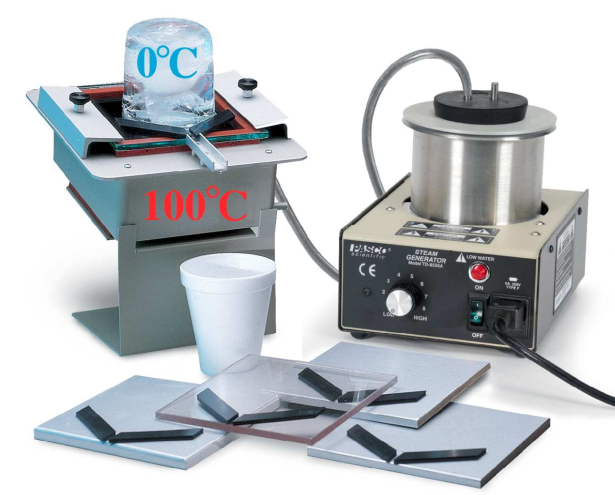
\includegraphics[width=1\linewidth]{img/montaje.png}
        \caption{Montaje usado. Tomado de  \cite{conductividad_notas}}
        \label{fig:montaje_a}
    \end{subfigure}
    \begin{subfigure}[b]{0.45\textwidth}
        \centering
        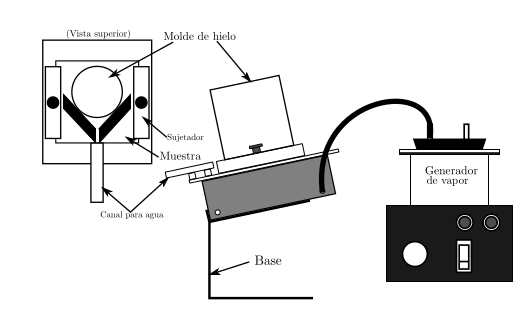
\includegraphics[width=\linewidth]{img/montaje_vista_lateral.png}
        \caption{Vista lateral esquematica del montaje. }
        \label{fig:montaje_b}
    \end{subfigure}
    \caption{Foto y esquema del montaje. Tomado de  \cite{conductividad_notas}}
\end{figure}
El equipo a utilizar consta de las siguientes partes \cite{conductividad_notas}:
\begin{itemize}
    \item base
    \item cámara de vapor,
    \item generador de vapor
    \item molde de hielo
    \item Muestras de diferentes materiales.
\end{itemize}
\section{Resultados y análisis}

\begin{figure}[htbp]
    \centering
    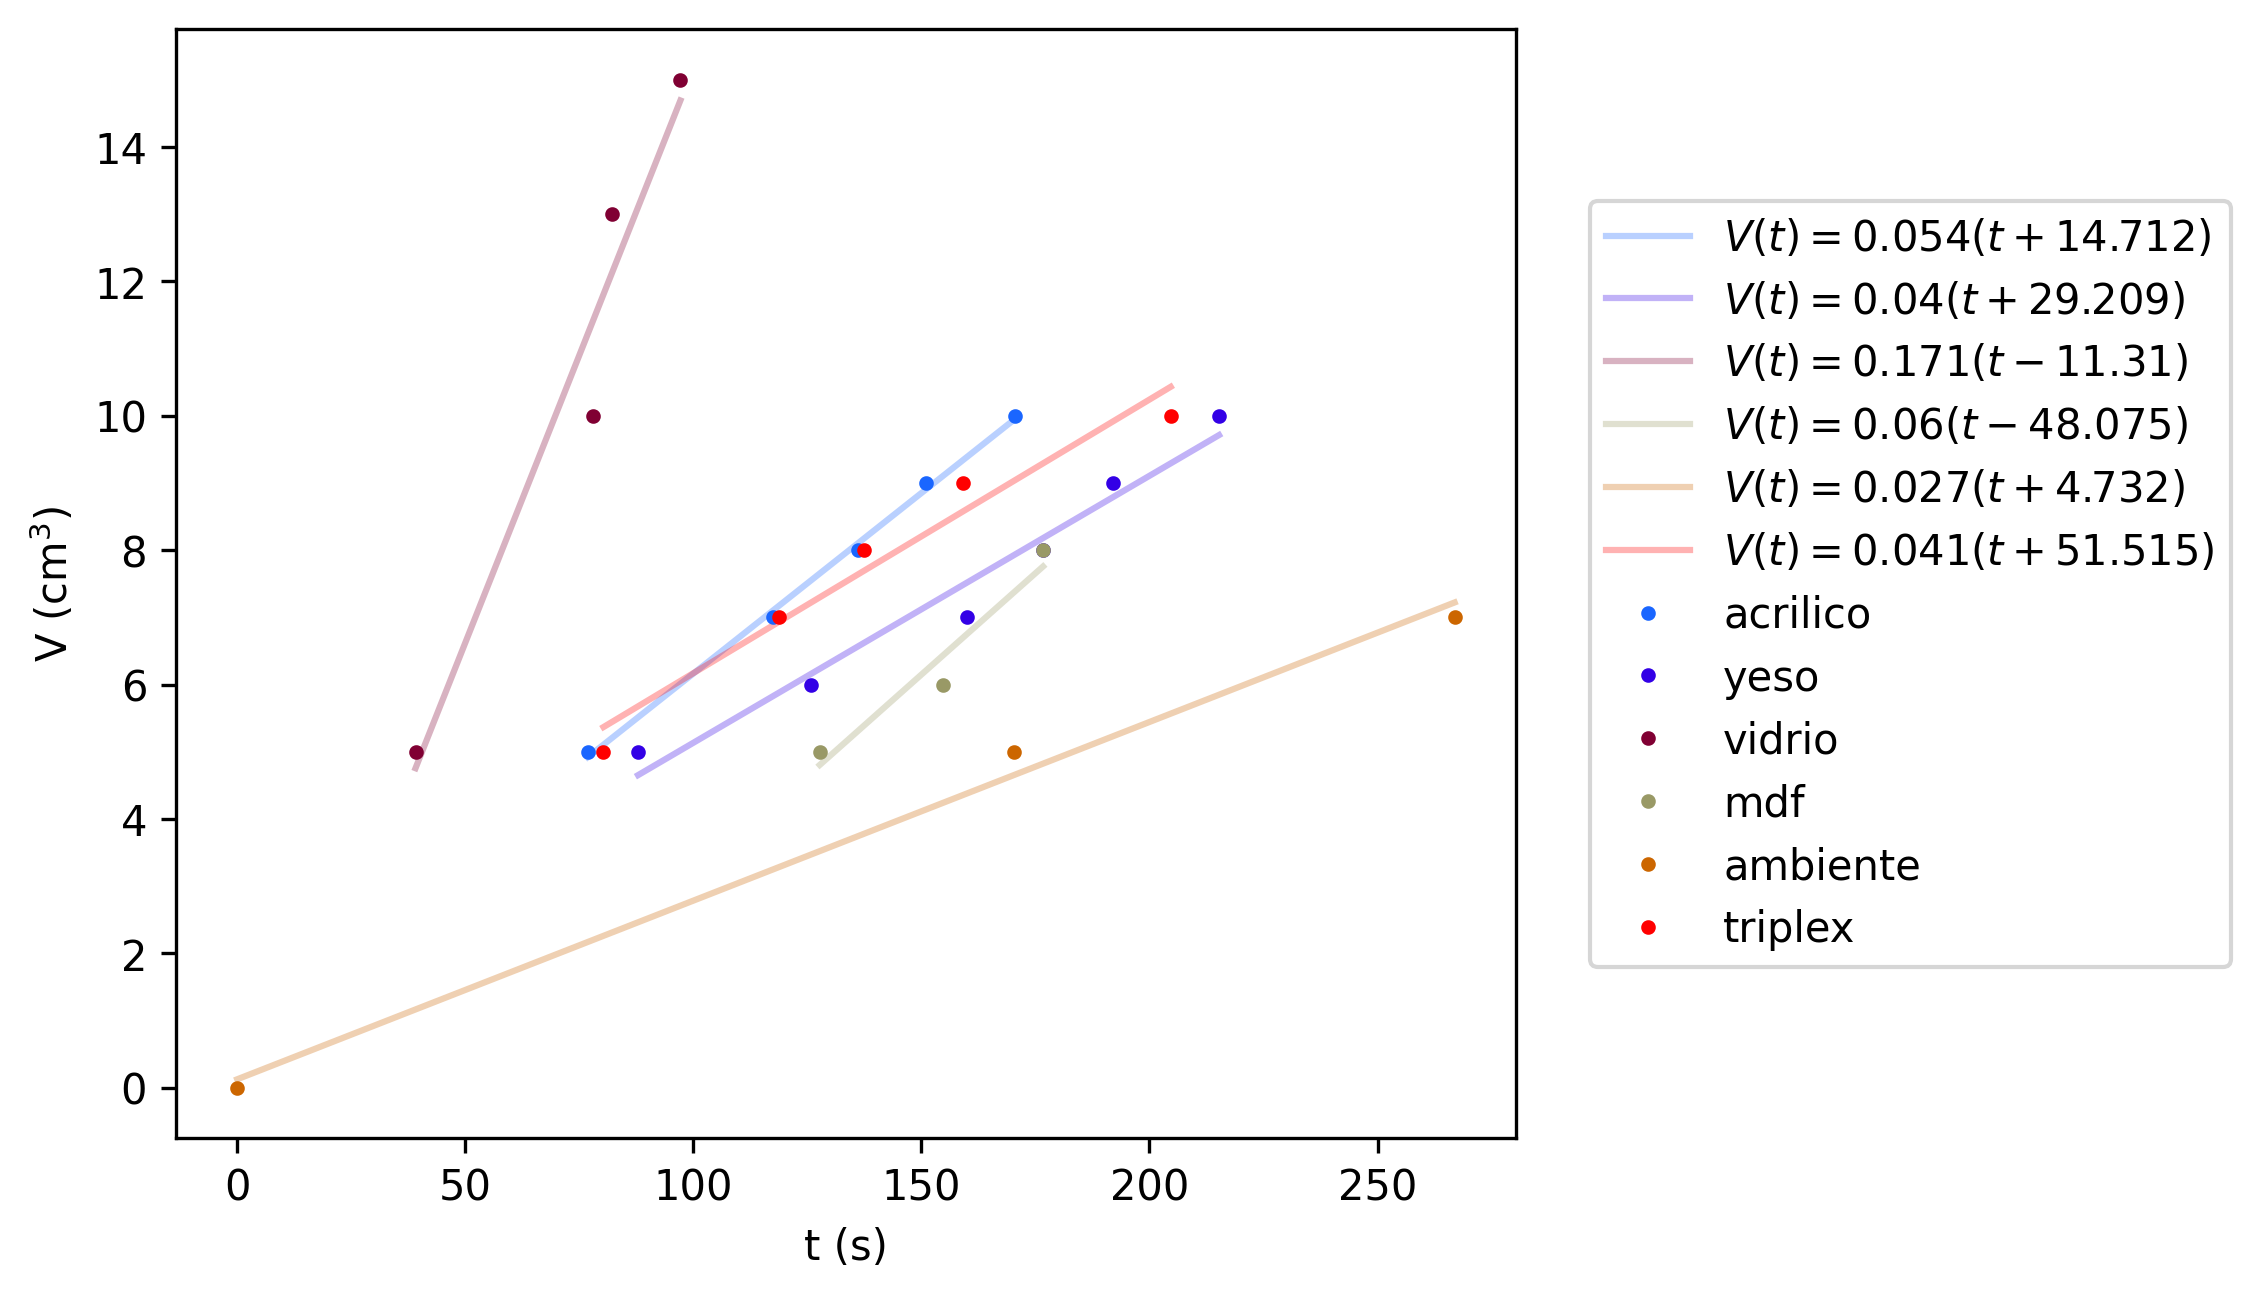
\includegraphics[width=0.5\linewidth]{img/V_vs_t.png}
    \caption{Volumen de hielo fundido como función del tiempo}
    \label{fig:V_vs_t}
\end{figure}

\section{Conclusiones}

%\end{multicols}
\printbibliography
\end{document}